\section{Feasibility Study (Technical,Economical,Operational)}
Feasibility study is made to see if the project on completion will serve the purpose of the organization for the amount of work, effort and the time that spend on it. Feasibility study lets the developer foresee the future of the project and the usefulness. A feasibility study of a system proposal is according to its workability, which is the impact on the organization, ability to meet their user needs and effective use of resources. Carrying out a feasibility study involves information assessment, information collection and report writing. The information assessment phase identifies the information that is required to answer the three questions set out above. Once the information has been identified, you should question information sources to discover the answers to these questions Thus when a new application is proposed it normally goes through a feasibility study before it is approved for development.

A feasibility study is designed to provide an overview of the primary issues related to a business idea.  The purpose is to identify any “make or break” issues that would prevent your business from being successful in the marketplace. In other words, a feasibility study determines whether the business idea makes sense. A thorough feasibility analysis provides a lot of information necessary for the business plan.  For example, a good market analysis is necessary in order to determine the project’s feasibility.  This information provides the basis for the market section of the business plan.

The document provide the feasibility of the project that is being designed and lists various areas that were considered very carefully during the feasibility study of this project such as Technical, Economic and Operational feasibilities. Feasibility is defined as the practical extent to which a project can be performed successfully. To evaluate feasibility, a feasibility study is performed, which determines whether the solution considered to accomplish the requirements is practical and workable in the software. Information such as resource availability, cost estimation for software development, benefits of the software to the organization after it is developed and cost to be incurred on its maintenance are considered during the feasibility study. The objective of the feasibility study is to establish the reasons for developing the software that is acceptable to users, adaptable to change and conformable to established standards.

Objectives of feasibility study are listed below.
\begin{itemize}
	\item To analyze whether the software will meet organizational requirements
	\item To determine whether the software can be implemented using the current technology and within the specified budget and schedule
	\item To determine whether the software can be integrated with other existing software.
\end{itemize}

\subsection{Types of Feasibility}
Various types of feasibility that are commonly considered include technical feasibility, operational feasibility, and economic feasibility.

\subsubsection{Technical Feasibility}
Technical feasibility is one of the first studies that must be conducted after the project has been identified. In large engineering projects consulting agencies that have large
staffs of engineers and technicians conduct technical studies dealing with the projects. 

When writing a feasibility report, the following should be taken to consideration:
\begin{itemize}
	\item A brief description of the business to assess more possible factors which could affect the study
	\item The part of the business being examined
	\item The human and economic factor
	\item The possible solutions to the problem
\end{itemize}

The system must be evaluated from the technical point of view first. The assessment of this feasibility must be based on an outline design of the system requirement in the terms of input, output, programs and procedures. Having identified an outline system, the investigation must go on to suggest the type of equipment, required method developing the system, of running the system once it has been designed. Technical feasibility assesses the current resources (such as hardware and software) and technology, which are required to accomplish user requirements in the software within the allocated time and budget. For this, the software development team ascertains whether the current resources and technology can be upgraded or added in the software to accomplish specified user requirements. Technical feasibility also performs the following tasks.

\begin{itemize}
	\item Analyzes the technical skills and capabilities of the software development team members
	\item Determines whether the relevant technology is stable and established
	\item Ascertains that the technology chosen for software development has a large number of users so that they can be consulted when problems arise or improvements are required.
\end{itemize}

Technical issues raised during the investigation are:
\begin{itemize}
	\item Does the existing technology sufficient for the suggested one?
	\item Can the system expand if developed?
\end{itemize}

The project should be developed such that the necessary functions and performance are achieved within the constraints. The project is developed within latest technology. Through the technology may become obsolete after some period of time, due to the fact that never version of same software supports older versions, the system may still be used. So there are minimal constraints involved with this project. The system has been developed using Java the project is technically feasible for development.

\subsubsection{Economic Feasibility}
The purpose of the economic feasibility assessment is to determine the positive economic benefits to the organization that the proposed system will provide. It includes quantification and identification of all the benefits expected. This assessment typically involves a cost/ benefits analysis.

Software is said to be economically feasible if it focuses on the issues listed below.
\begin{itemize}
	\item Cost incurred on software development to produce long-term gains for an organization.
	\item Cost required to conduct full software investigation (such as requirements elicitation and requirements analysis).
	\item Cost of hardware, software, development team, and training.
\end{itemize}

The following are some of the important financial questions asked during preliminary investigation:
\begin{itemize}
	\item The costs conduct a full system investigation.
	\item The cost of the hardware and software.
	\item The benefits in the form of reduced costs or fewer costly errors.
\end{itemize}

Since the system is developed as part of project work, there is no manual cost to spend for the proposed system. Also all the resources are already available, it give an indication of the system is economically possible for development.

\subsubsection{Operational Feasibility}
If the system is not easy to operate, than operational process would be difficult. The operator of the system should be given proper training. The system should be made such that the user can interface the system without any problem.

Operational feasibility is a measure of how well a proposed system solves the problems, and takes advantage of the opportunities identified during scope definition and how it satisfies the requirements identified in the requirements analysis phase of system development. The operational feasibility assessment focuses on the degree to which the proposed development projects fits in with the existing business environment and objectives with regard to development schedule, delivery date, corporate culture, and existing business processes.

Operational feasibility also performs the following tasks.

\begin{itemize}
	\item Determines whether the problems anticipated in user requirements are of high priority.
	\item Determines whether the solution suggested by the software development team is acceptable.
	\item Analyzes whether users will adapt to a new software.
	\item Determines whether the organization is satisfied by the alternative solutions proposed by the software development team.
\end{itemize}

This includes the following questions:
\begin{itemize}
	\item Is there sufficient support for the users?
	\item Will the proposed system cause harm?
	\item The project would be beneficial because it satisfies the objectives when developed and installed. All behavioral aspects are considered carefully and conclude that the project is behaviorally feasible.
\end{itemize}

This system proposed will have a very user friendly interface, a naïve user will be able to understand the user interface in seconds. It’ll have basic yet intriguing interface with a list various pdf categories, fab button which indicates that pdf upload using it and many other functions which is easily understandable.

\section{Software Requirement Specification Document}
\subsection{Data Requirement}
For this project, no specific data collections were required, all that was needed for testing the project. Initial Pdf or Ebook was uploaded to check sytem works in right way or not.  

\subsection{Performance Requirement}
Basis on resource requirements, this application will be able to run on pretty low-end devices with 512MB of ram and 800Mhz processor.

\subsection{Functional Requirement}
The application will have different kind of functions like uploading Ebooks of various categories. User can download and share that uploaded content.  

\section{Intended User}
This Application is made for any user who wants or wish to share Pdf or Ebook of various categories. Easy platform for the user who love to read ebook instead of buying it. 

\section{Features}
\begin{itemize}
	\item Upload and share pdf easily.
	\item Arranging Pdf or Ebook in various categories.
	\item User have access to delete uploading content(content uploaded by him/her self only). 
	 \item Feedback option given so that user can share his views.
\end{itemize}

	 	
\section{Expected hurdles}
\begin{itemize}
\item An algorithm for working of feedback notification to admins is one of the biggest hurdle in the project.
\item Libraries for Android studio needs to be added into the imported from various sources such as GitHub, Firebase.
\item Dependencies of the different libraries used in the project.

\end{itemize}

\section{SDLC model to be used}
\subsection{Waterfall Model}
 
The Waterfall Model is referred as a linear-sequential life cycle model. It is very simple to understand and use. In a waterfall model, each phase must be completed before the next phase can begin and there is no overlapping in the phases.

The Waterfall model is the earliest SDLC approach that was used for software development.The waterfall Model illustrates the software development process in a linear sequential flow. This means that any phase in the development process begins only if the previous phase is complete. In this waterfall model, the phases do not overlap.

Waterfall approach was first SDLC Model to be used widely in Software Engineering to ensure success of the project. In "The Waterfall" approach, the whole process of software development is divided into separate phases. In this Waterfall model, typically, the outcome of one phase acts as the input for the next phase sequentially.

\begin{figure}[ht]
\centering
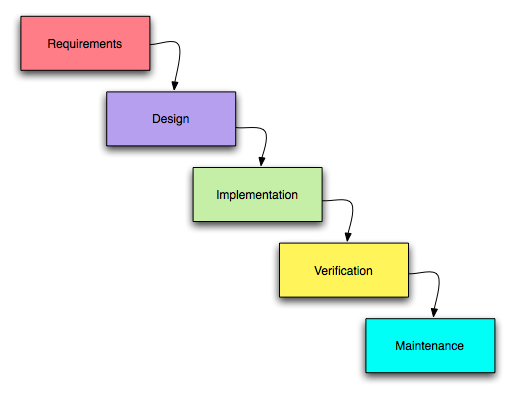
\includegraphics[scale=0.64]{images/waterfall.png}
\caption{Waterfall Model}
\end{figure}


%\newpage
